\documentclass[11pt,a4paper]{article}
\usepackage[a4paper,margin=2.2cm,top=2.2cm,bottom=2.4cm]{geometry}
\usepackage[T1]{fontenc}
\usepackage{lmodern}
\usepackage{amsmath,amssymb}
\usepackage{xcolor,enumitem,titlesec,graphicx,booktabs,float,caption,fancyhdr,array,tabularx}
\usepackage{listings}
\usepackage{tikz}\usetikzlibrary{arrows.meta,positioning}
\usepackage[hidelinks]{hyperref}
\definecolor{soft}{gray}{0.93}
\definecolor{acc}{HTML}{1F5FBF}
\titleformat{\section}{\large\bfseries}{}{0pt}{}[\titlerule]
\titlespacing*{\section}{0pt}{14pt}{6pt}
\titleformat{\subsection}{\normalsize\bfseries}{}{0pt}{}
\titlespacing*{\subsection}{0pt}{9pt}{3pt}
\setlength{\parindent}{0pt}
\setlength{\parskip}{5pt}
\setlist{nosep,leftmargin=1.5em,itemsep=3pt}
\pagestyle{fancy}\fancyhf{}
\renewcommand{\headrulewidth}{0pt}\renewcommand{\footrulewidth}{0.4pt}
\lfoot{KFUPM Controls \& Instrumentation}\cfoot{\thepage}\rfoot{Prof. Aamer Iqbal Bhatti}
\emergencystretch=3em
\sloppy
\captionsetup{font=small,labelfont=bf}
\lstset{basicstyle=\ttfamily\small,backgroundcolor=\color{soft},frame=none,columns=fullflexible,
  keepspaces=true,showstringspaces=false,xleftmargin=4pt,framexleftmargin=4pt,
  commentstyle=\color{gray}\itshape,language=Python,escapeinside={(*}{*)}}

\begin{document}

\begin{center}
{\LARGE\bfseries SCE 672: Advanced Robotics}\\[5pt]
{\large\bfseries Assessment 2 Presentation: Flatness-Based Chase of AprilTag 3}
\end{center}
\noindent\textbf{Student:} Ameen Ur Rehman (202527430)\\
\textbf{Instructor:} Prof. Aamer Iqbal Bhatti\\
\textbf{Code:} \url{https://github.com/AmeenUrRehman/RoboMaster-Advanced-Robotics}\\
\textbf{Folder:} \texttt{Assignment 2}
\par\vspace{2pt}\noindent\rule{\linewidth}{0.8pt}

\textbf{In one sentence:} a RoboMaster EP finds AprilTag~3, turns to face it, drives a smooth planned path to it, and stops about 20\,cm in front of it.
This document follows the five presentation points in order: (1) the planned path in the GitHub code, (2) where the command is sent to the robot, (3) the reference graphs of velocity and $x$, (4) the tracking errors, and (5) the video.
All numbers come from the code and from the final run's log (\texttt{logs/flat\_run5/motor\_voltage\_log.csv}).

% ---------------------------------------------------------------------------------------
\section{Words to know}
\begin{center}\small
\begin{tabularx}{\linewidth}{@{}>{\bfseries}p{3.6cm}X@{}}
\toprule
\textnormal{\textbf{Word}} & \textbf{Plain meaning}\\
\midrule
RoboMaster EP & The small DJI robot with four mecanum wheels and a camera.\\
AprilTag & A printed black-and-white square, like a simple QR code. The robot follows \textbf{Tag~3}; Tags 1 and 2 are decoys.\\
ROS 2 & The software ``post office'': programs send each other messages on named channels called \emph{topics}.\\
\texttt{cmd\_vel} & The topic that carries the drive order to the robot: forward speed $v$ and turn rate $\omega$.\\
$v$ & Forward speed, in metres per second (m/s).\\
$\omega$ (omega) & Turning speed, in radians per second (rad/s). $\omega=0$ means drive straight.\\
$x$ & How far the robot has driven forward since the chase started (m).\\
$d_0$ & Distance from the robot to the tag when the chase starts: 1.053\,m in the real run.\\
$T$ & Time the plan allows for the whole chase: 8.53\,s in the real run.\\
Reference & What the plan says the robot \emph{should} do at each moment.\\
Tracking error & Where the robot really is minus where the plan says it should be.\\
Differential flatness & If we plan only the position $(x,y)$ over time, the speed $v$ and turn rate $\omega$ follow from a simple formula. No heavy optimisation is needed.\\
Cubic polynomial & A smooth curve $a_0+a_1t+a_2t^2+a_3t^3$: it starts and ends gently, with no jerks.\\
Standoff & The gap left in front of the tag at the end: 0.20\,m.\\
\bottomrule
\end{tabularx}
\end{center}

% ---------------------------------------------------------------------------------------
\section{The big picture}
\begin{figure}[H]\centering
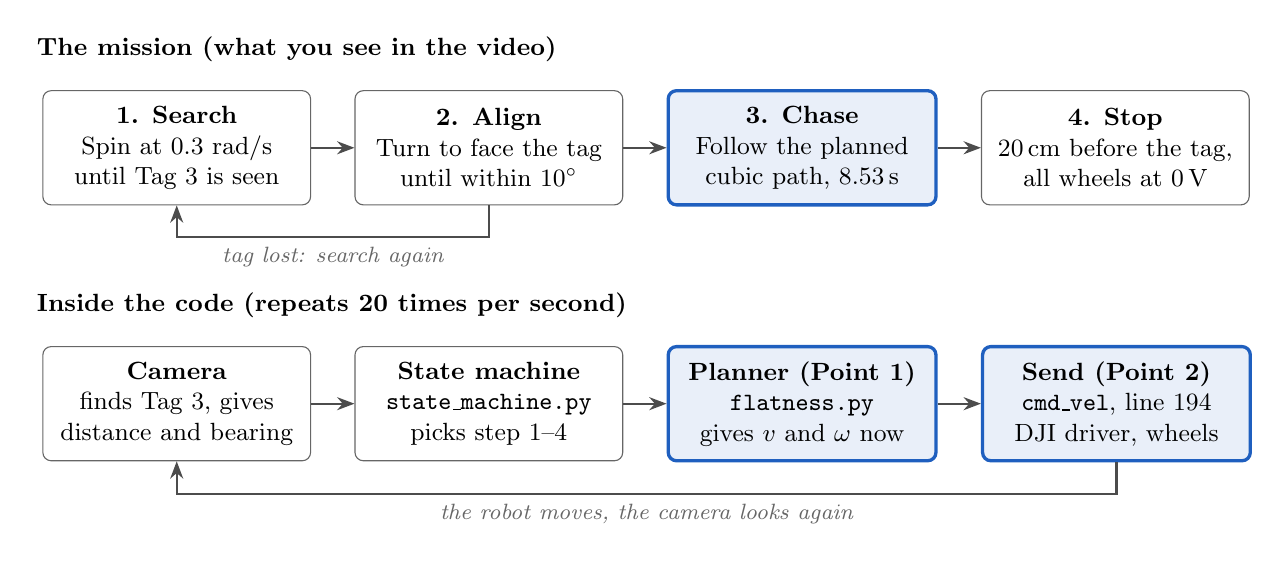
\begin{tikzpicture}[
  box/.style={draw=black!60,rounded corners=3pt,minimum width=3.4cm,minimum height=1.45cm,align=center,font=\small},
  key/.style={box,draw=acc,line width=1.2pt,fill=acc!10},
  arr/.style={-{Stealth[length=2.2mm]},black!70,thick},
  note/.style={font=\footnotesize\itshape,text=black!60}]
\node[font=\small\bfseries,anchor=west] at (-1.9,1.25) {The mission (what you see in the video)};
\node[box] (s) at (0,0) {\textbf{1. Search}\\Spin at 0.3 rad/s\\until Tag 3 is seen};
\node[box,right=0.55cm of s] (a) {\textbf{2. Align}\\Turn to face the tag\\until within $10^\circ$};
\node[key,right=0.55cm of a] (c) {\textbf{3. Chase}\\Follow the planned\\cubic path, 8.53\,s};
\node[box,right=0.55cm of c] (p) {\textbf{4. Stop}\\20\,cm before the tag,\\all wheels at 0\,V};
\draw[arr] (s) -- (a); \draw[arr] (a) -- (c); \draw[arr] (c) -- (p);
\draw[arr] (a.south) -- ++(0,-0.4) -| node[note,pos=0.25,below]{tag lost: search again} (s.south);
\node[font=\small\bfseries,anchor=west] at (-1.9,-2.0) {Inside the code (repeats 20 times per second)};
\node[box] (cam) at (0,-3.25) {\textbf{Camera}\\finds Tag 3, gives\\distance and bearing};
\node[box,right=0.55cm of cam] (fsm) {\textbf{State machine}\\\texttt{state\_machine.py}\\picks step 1--4};
\node[key,right=0.55cm of fsm] (pl) {\textbf{Planner (Point 1)}\\\texttt{flatness.py}\\gives $v$ and $\omega$ now};
\node[key,right=0.55cm of pl] (pub) {\textbf{Send (Point 2)}\\\texttt{cmd\_vel}, line 194\\DJI driver, wheels};
\draw[arr] (cam) -- (fsm); \draw[arr] (fsm) -- (pl); \draw[arr] (pl) -- (pub);
\draw[arr] (pub.south) -- ++(0,-0.4) -| node[note,pos=0.25,below]{the robot moves, the camera looks again} (cam.south);
\end{tikzpicture}
\caption{Top: the four steps of the mission. Bottom: the loop the code runs every 0.05\,s. The blue boxes are presentation Points 1 and 2.}
\end{figure}

\subsection*{The four steps in detail: when does the robot switch?}
The file \texttt{state\_machine.py} decides which step the robot is in. Each arrow below is a rule in that file, with its real number.
\begin{figure}[H]\centering
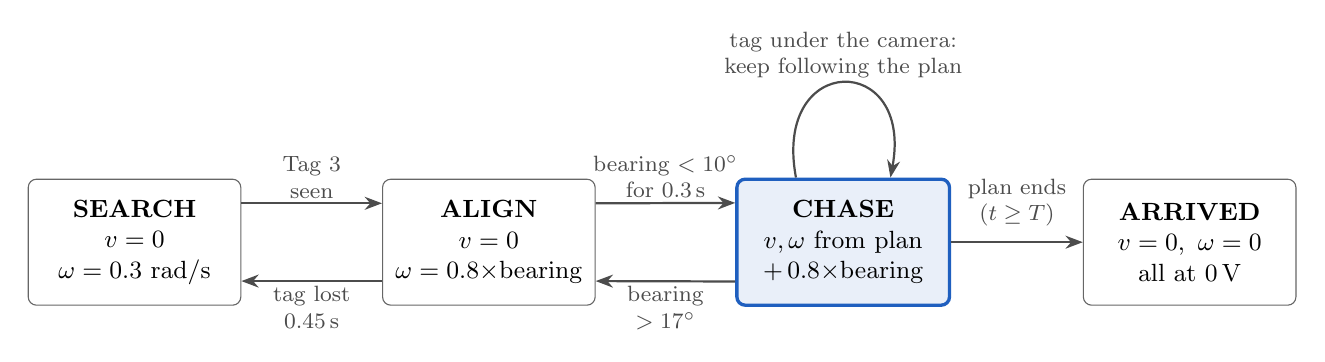
\begin{tikzpicture}[
  st/.style={draw=black!60,rounded corners=3pt,minimum width=2.7cm,minimum height=1.6cm,align=center,font=\small},
  key/.style={st,draw=acc,line width=1.2pt,fill=acc!10},
  arr/.style={-{Stealth[length=2.2mm]},black!70,thick},
  lab/.style={font=\footnotesize,align=center,inner sep=1.5pt}]
\node[st]  (S) at (0,0)    {\textbf{SEARCH}\\$v=0$\\$\omega=0.3$ rad/s};
\node[st]  (A) at (4.5,0)  {\textbf{ALIGN}\\$v=0$\\$\omega=0.8\times$bearing};
\node[key] (C) at (9.0,0)  {\textbf{CHASE}\\$v,\omega$ from plan\\$+\,0.8\times$bearing};
\node[st]  (R) at (13.4,0) {\textbf{ARRIVED}\\$v=0,\ \omega=0$\\all at 0\,V};
\draw[arr] (S.20) -- node[lab,above]{Tag 3\\seen} (A.160);
\draw[arr] (A.200) -- node[lab,below]{tag lost\\0.45\,s} (S.340);
\draw[arr] (A.20) -- node[lab,above]{bearing $<10^\circ$\\for 0.3\,s} (C.160);
\draw[arr] (C.200) -- node[lab,below]{bearing\\$>17^\circ$} (A.340);
\draw[arr] (C) -- node[lab,above=4pt]{plan ends\\($t\ge T$)} (R);
\draw[arr] ([xshift=-6mm]C.north) .. controls +(-0.3,1.6) and +(0.3,1.6) .. node[lab,above]{tag under the camera:\\keep following the plan} ([xshift=6mm]C.north);
\end{tikzpicture}
\caption{The state machine. ``Bearing'' is the angle between the camera's centre line and the tag. Once chasing, the robot keeps following the plan even when the floor tag goes under the camera (tag last seen within 1.8\,m). The code also stops at once if the camera or the ToF sensor reads 0.20\,m or less; in the final run the stop came from the plan ending.}
\end{figure}

% ---------------------------------------------------------------------------------------
\section{Point 1: How the path is planned (GitHub code)}
The path is a smooth straight line to 20\,cm in front of the tag. It is planned once, at the moment the chase starts.
File: \texttt{Assignment 2/rm\_flatness\_nav/rm\_flatness\_nav/flatness.py}.

\begin{figure}[H]\centering
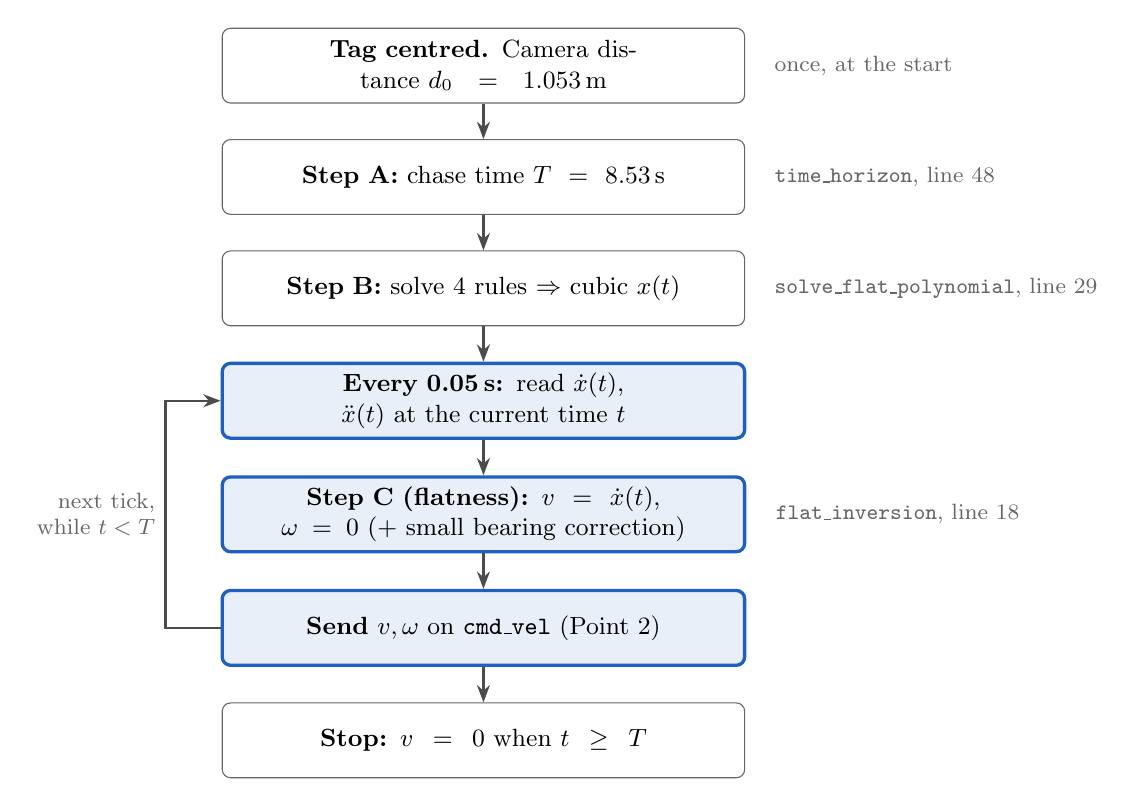
\begin{tikzpicture}[
  b/.style={draw=black!60,rounded corners=3pt,text width=6.4cm,minimum height=0.95cm,align=center,font=\small},
  k/.style={b,draw=acc,line width=1.2pt,fill=acc!10},
  arr/.style={-{Stealth[length=2.2mm]},black!70,thick},
  side/.style={font=\footnotesize,text=black!60,align=left,anchor=west},
  node distance=0.45cm]
\node[b] (n1) {\textbf{Tag centred.} Camera distance $d_0=1.053$\,m};
\node[b,below=of n1] (n2) {\textbf{Step A:} chase time $T=8.53$\,s};
\node[b,below=of n2] (n3) {\textbf{Step B:} solve 4 rules $\Rightarrow$ cubic $x(t)$};
\node[k,below=of n3] (n4) {\textbf{Every 0.05\,s:} read $\dot x(t)$, $\ddot x(t)$ at the current time $t$};
\node[k,below=of n4] (n5) {\textbf{Step C (flatness):} $v=\dot x(t)$,\ $\omega=0$ (+ small bearing correction)};
\node[k,below=of n5] (n6) {\textbf{Send} $v,\omega$ on \texttt{cmd\_vel} (Point 2)};
\node[b,below=of n6] (n7) {\textbf{Stop:} $v=0$ when $t\ge T$};
\foreach \a/\c in {n1/n2,n2/n3,n3/n4,n4/n5,n5/n6,n6/n7} \draw[arr] (\a) -- (\c);
\draw[arr] (n6.west) -- ++(-0.7,0) |- node[side,pos=0.25,left,anchor=east,align=right]{next tick,\\while $t<T$} (n4.west);
\node[side] at ([xshift=0.25cm]n1.east) {once, at the start};
\node[side] at ([xshift=0.25cm]n2.east) {\texttt{time\_horizon}, line 48};
\node[side] at ([xshift=0.25cm]n3.east) {\texttt{solve\_flat\_polynomial}, line 29};
\node[side] at ([xshift=0.25cm]n5.east) {\texttt{flat\_inversion}, line 18};
\end{tikzpicture}
\caption{The planner at a glance. White boxes run once when the chase starts; blue boxes repeat 20 times per second until the plan ends.}
\end{figure}

\subsection*{Step A: How long should the chase take? \quad(\texttt{time\_horizon}, line 48)}
\[
T=\max\!\left(4.0,\ \frac{1.6\,(d_0-0.20)}{v_{\max}}\right),\qquad v_{\max}=0.16\ \text{m/s}.
\]
Real run: $d_0=1.053$\,m, so $T=1.6\times0.853/0.16=\mathbf{8.53\,s}$. A farther tag gets more time, so the top speed stays about 0.137\,m/s.

\subsection*{Step B: Draw a smooth curve for $x(t)$ \quad(\texttt{solve\_flat\_polynomial}, line 29)}
The curve $x(t)=a_0+a_1t+a_2t^2+a_3t^3$ must obey four rules:
\begin{center}\small
\begin{tabular}{@{}ll@{}}
\toprule
\textbf{Rule} & \textbf{Meaning}\\
\midrule
$x(0)=0$ & start where the robot is now\\
$\dot x(0)=0.06$ m/s & start with a small speed\\
$x(T)=d_0-0.20=0.853$ m & end 20\,cm before the tag\\
$\dot x(T)=0$ & arrive with zero speed\\
\bottomrule
\end{tabular}
\end{center}
Four rules and four unknowns: the code solves them with \texttt{numpy.linalg.solve}. Result for the real run:
\[
x(t)=0.06\,t+0.0211\,t^2-0.00192\,t^3 .
\]
The sideways curve $y(t)$ is zero, because the robot first turns to face the tag.

\subsection*{Step C: Turn the curve into driving orders (flatness) \quad(\texttt{flat\_inversion}, line 18)}
\[
v=\sqrt{\dot x^2+\dot y^2},\qquad \omega=\frac{\dot x\,\ddot y-\dot y\,\ddot x}{\dot x^2+\dot y^2}.
\]
With $y=0$ this gives $v=\dot x(t)$ (the slope of the curve) and $\omega=0$ (drive straight). No optimiser is used, only this formula.

\begin{lstlisting}
def solve_flat_polynomial(z0, zdot0, zf, zdotf, T):     # flatness.py, line 29
    A = np.array([[1.0, 0.0, 0.0,    0.0],
                  [0.0, 1.0, 0.0,    0.0],
                  [1.0, T,   T**2,   T**3],
                  [0.0, 1.0, 2.0*T,  3.0*T**2]])
    b = np.array([z0, zdot0, zf, zdotf], dtype=float)
    return np.linalg.solve(A, b)                         # [a0, a1, a2, a3]
\end{lstlisting}
% ---------------------------------------------------------------------------------------
\section{Point 2: Where the command is sent to the RoboMaster}
The command leaves the code in one place: \texttt{nav\_node.py}, function \texttt{tick()}, which publishes on the \texttt{cmd\_vel} topic 20 times per second.
\begin{lstlisting}
# nav_node.py, line 103: create the "mailbox" to the robot
self.cmd_pub = self.create_publisher(Twist, 'cmd_vel', 10)

# nav_node.py, lines 190-194: runs every 0.05 s (20 Hz)
v, w = self.fsm.update(obs)                 # the plan gives speed v and turn w
tw = Twist()
tw.linear.x, tw.angular.z = float(v), float(w)
self.cmd_pub.publish(tw)                    # (*\textbf{<-- sent to the RoboMaster here}*)
\end{lstlisting}
The chain, step by step:
\begin{enumerate}
  \item \texttt{tick()} runs 20 times per second (\texttt{control\_rate = 20}).
  \item It asks the state machine for $v$ and $\omega$. During the chase this is \texttt{\_chase()} in \texttt{state\_machine.py} (line 131), which reads the planned curve at the current time with \texttt{self.traj.sample(t)}.
  \item It packs $v$ and $\omega$ into a \texttt{Twist} message and publishes it on \texttt{cmd\_vel}.
  \item DJI's \texttt{robomaster\_ros} driver (started with \texttt{ros2 launch robomaster\_ros ep.launch conn\_type:=rndis}) listens on \texttt{cmd\_vel} and sends the speeds over the USB cable.
  \item The robot's own controller turns the four wheels.
\end{enumerate}
Safety: when the plan ends, or Ctrl+C is pressed, the node sends zero speed (\texttt{shutdown()}, line 225), so the robot always stops.
% ---------------------------------------------------------------------------------------
\section{Point 3: Reference graphs of velocity and $x$}
The reference starts at 0.06\,m/s, peaks at 0.137\,m/s in the middle, and reaches zero exactly when $x$ reaches 0.853\,m at $T=8.53$\,s.
\begin{figure}[H]\centering
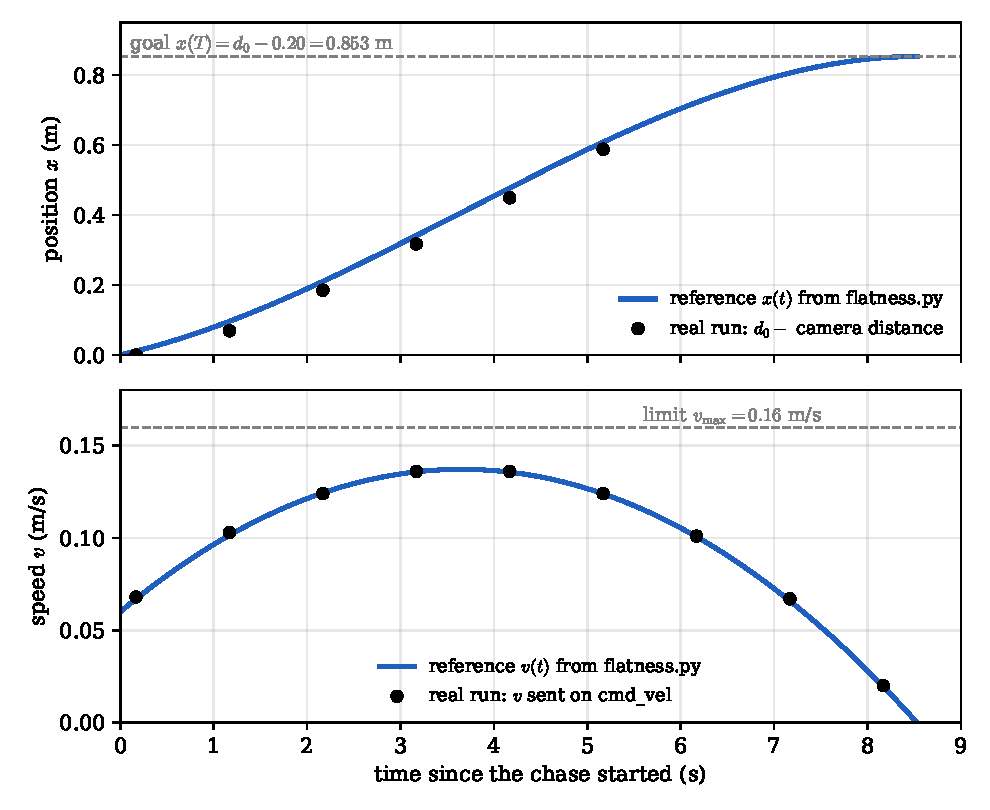
\includegraphics[width=0.92\linewidth]{fig_reference.pdf}
\caption{Blue lines: the reference computed by \texttt{flatness.py} for $d_0=1.053$\,m. Dots: the real run (1 sample per second). Top: position; the dots are $d_0$ minus the camera distance to the tag. Bottom: speed; the dots are the values sent on \texttt{cmd\_vel}. Time zero is the start of the chase (9.83\,s in the log).}
\end{figure}
\textbf{How to read it.} The top curve is S-shaped: slow start, fast middle, gentle stop. The bottom curve is its slope (the speed): a hill that never reaches the dashed 0.16\,m/s limit.
% ---------------------------------------------------------------------------------------
\section{Point 4: Tracking errors}
The robot stayed within \textbf{3\,cm} of the planned position and within \textbf{4$^\circ$} of the tag's direction. It ran slightly behind the plan.

\textbf{How it is measured.} The camera measures the distance to the tag in every frame, so
\[
x_{\text{real}}=d_0-\text{camera distance},\qquad \text{tracking error}=x_{\text{real}}-x_{\text{plan}}.
\]
\begin{center}\small
\begin{tabular}{@{}cccrc@{}}
\toprule
\textbf{Time in log (s)} & \textbf{Planned $x$ (m)} & \textbf{Real $x$ (m)} & \textbf{Position error (cm)} & \textbf{Heading error (deg)}\\
\midrule
10 & 0.011 & 0.000 & $-1.1$ & 3.9\\
11 & 0.096 & 0.069 & $-2.7$ & 1.0\\
12 & 0.210 & 0.185 & $-2.5$ & 0.2\\
13 & 0.341 & 0.317 & $-2.4$ & 0.3\\
14 & 0.478 & 0.449 & $-2.9$ & 0.7\\
15 & 0.608 & 0.588 & $-2.0$ & 0.4\\
\bottomrule
\end{tabular}
\end{center}
\begin{figure}[H]\centering
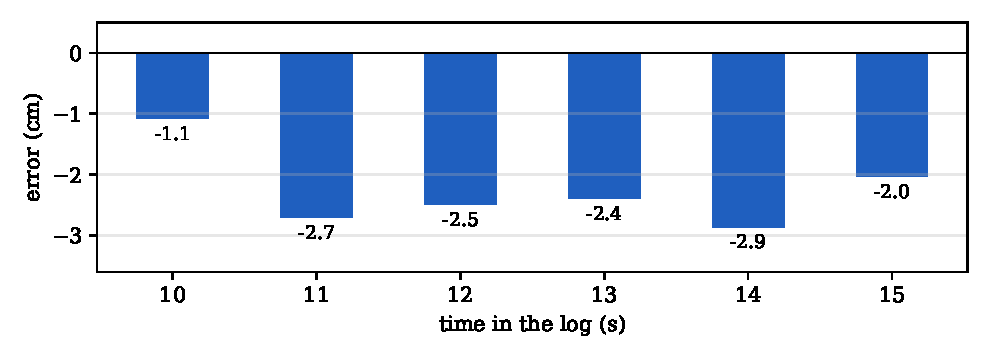
\includegraphics[width=0.85\linewidth]{fig_error.pdf}
\caption{Position tracking error at each logged second. Minus means the robot was slightly behind the plan.}
\end{figure}
\textbf{End point:} planned gap 20\,cm, real gap about 20\,cm (measured by hand).

\textbf{Why the error is small.} The robot first turns to face the tag, so the path is a straight line. While the tag is visible, a small correction ($0.8\times$ bearing) is added to $\omega$.

\subsection*{Why the robot still stops at about 20\,cm}
\begin{itemize}
  \item \textbf{The error is small next to the path.} The robot was 1 to 3\,cm behind the plan on a path of 85\,cm, about 2 to 3\%. A gap of ``about 20\,cm'' measured by hand cannot separate 20 from 22\,cm.
  \item \textbf{The robot finishes the plan by itself.} After 15\,s in the log the floor tag is too close to see (it is under the camera). The code keeps sending the planned speeds until $T=8.53$\,s is over, then sends zero. So the robot drives the whole planned 0.853\,m.
  \item \textbf{Part of the ``error'' may come from the camera.} The camera does not measure distance directly. It computes it from the tag's size in the image and from the camera's downward tilt (about $20^\circ$, read from the images). A small error in the tag size or the tilt shifts every distance by a centimetre or two, which looks like a lag. The robot may therefore have been even closer to the plan than the table shows.
\end{itemize}
\begin{figure}[H]\centering
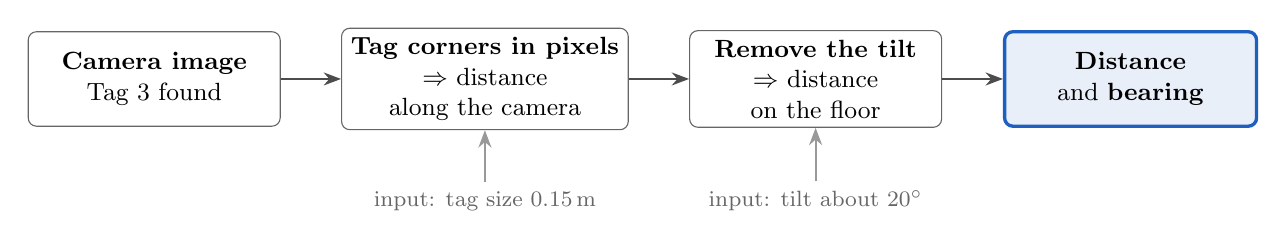
\begin{tikzpicture}[
  b/.style={draw=black!60,rounded corners=3pt,minimum width=3.2cm,minimum height=1.2cm,align=center,font=\small},
  k/.style={b,draw=acc,line width=1.2pt,fill=acc!10},
  arr/.style={-{Stealth[length=2.2mm]},black!70,thick},
  inp/.style={font=\footnotesize,text=black!60,align=center}]
\node[b] (img) at (0,0) {\textbf{Camera image}\\Tag 3 found};
\node[b] (pose) at (4.2,0) {\textbf{Tag corners in pixels}\\$\Rightarrow$ distance\\along the camera};
\node[b] (tilt) at (8.4,0) {\textbf{Remove the tilt}\\$\Rightarrow$ distance\\on the floor};
\node[k] (out) at (12.4,0) {\textbf{Distance}\\and \textbf{bearing}};
\draw[arr] (img) -- (pose); \draw[arr] (pose) -- (tilt); \draw[arr] (tilt) -- (out);
\node[inp] (s) at (4.2,-1.55) {input: tag size 0.15\,m};
\node[inp] (t) at (8.4,-1.55) {input: tilt about $20^\circ$};
\draw[arr,black!40] (s) -- (pose); \draw[arr,black!40] (t) -- (tilt);
\end{tikzpicture}
\caption{How the camera turns an image into a distance (\texttt{tag\_detector.py}). The two grey inputs are set by hand, so a small error in either shifts the measured distance.}
\end{figure}
% ---------------------------------------------------------------------------------------
\section{Point 5: Video}
The demonstration videos (each 45\,s or less) show the four steps of the mission.
\begin{itemize}
  \item Video 1: \url{https://youtu.be/EaZKQfd3usE}
  \item Video 2: \url{https://youtu.be/JlHnuVnLLrA}
\end{itemize}
\begin{enumerate}
  \item \textbf{Search}: the robot turns on the spot until it sees Tag 3.
  \item \textbf{Align}: it turns to face the tag.
  \item \textbf{Chase}: it follows the planned path: slow start, faster middle, slow end.
  \item \textbf{Stop}: it stops about 20\,cm before the tag with all wheel voltages at 0\,V.
\end{enumerate}

\end{document}
